% =====================================================================
% Chelina's part: genre labels, genre network and the network analysis
% (notebooks/analysis.ipynb, Steps 1-8). First draft, longer than the
% final version so it can be cut down.
%
% Needs in the preamble:  \usepackage{graphicx, booktabs, amsmath}
% Figures are read from figures/*.pdf (copy them next to the .tex file
% or change the paths).
% All \cite keys starting with TODO_ are placeholders for the .bib file.
%
% Macros (move to the preamble if the teammates use them too):
\newcommand{\Glyr}{\ensuremath{G_{\mathrm{lyrics}}}}
\newcommand{\Ginst}{\ensuremath{G_{\mathrm{instruments}}}}
\newcommand{\Gcomb}{\ensuremath{G_{\mathrm{combined}}}}
% =====================================================================


% =====================================================================
\section*{Results}
% =====================================================================

Three networks of songs first released 1970--1980 were built, each from a different description of a song (Materials and Methods). In \Glyr, 7,682 songs are linked by the cosine similarity of their TF-IDF lyric vectors. In \Ginst, 2,171 songs are linked by the instrument families they share (14 families, weighted so that a family on many songs counts little). In \Gcomb, the 1,428 songs with lyrics, instruments and country are linked through shared instrument families, release country and characteristic lyric words, with equal total weight for the three types. Genre is never used to build an edge. Instead, the communities are compared afterwards with a vote-based genre from MusicBrainz user tags, reduced to nine broad classes (rock, r\&b, pop, country, reggae, folk, electronic, jazz and other), and with release country. Each graph was first reduced to its statistically significant edges with the disparity filter, and communities were found with Louvain on the largest connected component (LCC) of this backbone.

\subsection*{Genre labels}
Before the main analysis, the labels themselves were examined in a genre network, where songs are linked by the MusicBrainz genre tags they share. This network (16,463 songs, 106,027 edges) has a modularity of 0.638 for its greedy-modularity communities, against 0.402 when the primary genres are used as communities. The multi-label tag lists therefore group songs more tightly than a single primary genre does, and part of the genre information is lost when a song is reduced to one label. Of the 2,926 communities, 2,766 are single songs whose genres were not sampled into any edge, while 81\% of the songs fall in 20 communities of at least 20 songs. These large communities mix related genres: the largest (2,428 songs) is 32\% soul, 16\% rock, 12\% jazz and 10\% funk, and the country community (1,729 songs) is 44\% country and 19\% rock.

\subsection*{All three graphs have community structure beyond their degrees}
The disparity filter kept 3.9\% of the edges of \Glyr{} (992,571 edges, LCC 7,681 songs), 4.8\% of \Gcomb{} (46,399 edges, all 1,428 songs) and 2.5\% of \Ginst{} (54,248 edges). In \Ginst, 1,200 of the 2,171 songs lost all their edges, leaving an LCC of 971 songs. These are songs with only a standard line-up, such as bass, drums and guitar (385 songs) or bass, drums, guitar and keys (250 songs). Such a song is about equally similar to every other song, so none of its edges stands out. Songs with a less common family, such as synth, organ or folk strings, stay in the LCC. The backbones cluster 2.5 to 3.6 times more than their configuration-model expectation (average clustering 0.124, 0.786 and 0.301 for \Glyr, \Ginst{} and \Gcomb).

Louvain found 6 communities in \Glyr{} (largest 2,366 songs), 7 in \Ginst{} (largest 276) and 20 in \Gcomb{} (largest 154). The modularity of all three partitions is far above that of the degree-preserving null graphs (Fig.~1, left column): $M = 0.212$ against $0.055 \pm 0.001$ for \Glyr{} ($z = 184$), $0.482$ against $0.067 \pm 0.001$ for \Ginst{} ($z = 337$) and $0.371$ against $0.180 \pm 0.001$ for \Gcomb{} ($z = 195$). No null graph reached the real value ($p = 0.0099$, the minimum for 100 nulls). The partitions differ in how stable they are. Agreement between two partitions is measured here and below with the adjusted mutual information (AMI), which is 0 for chance agreement and 1 for identical partitions. The mean pairwise AMI over 20 Louvain seeds is 0.90 for \Ginst, 0.62 for \Glyr{} and 0.58 for \Gcomb. In \Glyr{} and \Gcomb{} individual songs change community between seeds, while $M$ and the AMI with genre hardly change ($M = 0.211 \pm 0.002$ and AMI $= 0.029 \pm 0.002$ for \Glyr).

\begin{figure}[t]
  \centering
  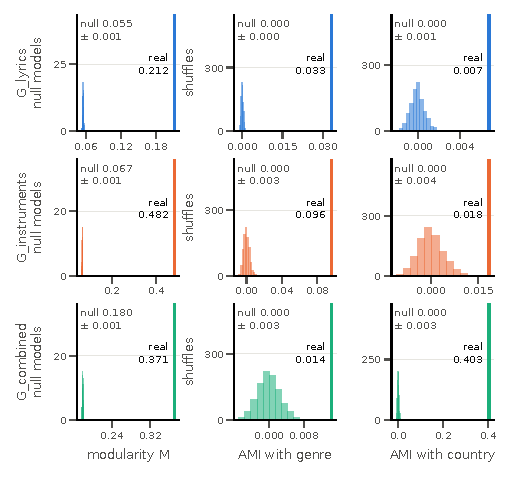
\includegraphics[width=\linewidth]{figures/report_null_checks.pdf}
  \caption{\textbf{The communities are genuine, but they share little information with genre.} One row per graph. Left column: Louvain modularity $M$ of the backbone (vertical line) against $M$ of 100 degree-preserving rewirings of the same backbone (histogram, mean $\pm$ sd in the corner). No rewired graph comes close in any of the three graphs. Middle and right columns: adjusted mutual information (AMI) between the communities and the genre (vote-based MusicBrainz class) or the release country, against 1,000 shuffles of the labels over the songs (histogram). All real values are above every shuffle ($p = 0.001$). The AMI with genre is 0.033 for lyrics, 0.096 for instruments and 0.014 for the combined graph, which agrees 28 times better with release country (0.403). Note the different $x$-axes.}
  \label{fig:nulls}
\end{figure}

\subsection*{The communities only weakly match established genres}
Although the structure is genuine, the communities are not genres (Fig.~1, middle column; Table~1). The AMI with genre is 0.033 for \Glyr, 0.014 for \Gcomb{} and 0.096 for \Ginst. All three are above every label shuffle ($p = 0.001$), so the agreement is weak but not random. The other measures agree. Genre assortativity, which measures whether edges join songs of the same genre more often than chance, is 0.043, 0.035 and 0.076, and genre used as a partition reaches a modularity of only 0.033, 0.020 and 0.047, against 0.207, 0.371 and 0.485 for Louvain on the same songs. On the 673 songs common to all three graphs, the AMI with genre is 0.030 (\Glyr), 0.026 (\Gcomb) and 0.087 (\Ginst), so the ranking does not come from the different song sets. Using the primary core genre instead of the coarse class gives similar values (0.035, 0.021 and 0.092).

The composition of the communities shows why (Fig.~2, left). Rock is 57\% of the labeled songs in \Glyr, 67\% in \Ginst{} and 79\% in \Gcomb, and it is the largest genre in every community. In \Glyr, the largest deviations from the baseline are communities 2 and 3, with 34\% and 32\% r\&b against 18\% overall. The instrument communities depart more. Community 2 of \Ginst{} is 36\% country (baseline 8\%), and community 1 is 17\% r\&b and 9\% jazz (baseline 8\% and 3\%).

\begin{figure}[t]
  \centering
  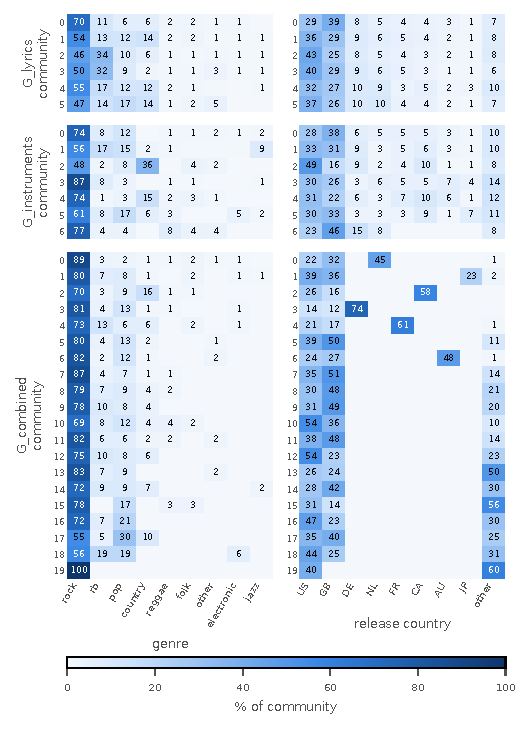
\includegraphics[width=\linewidth]{figures/report_heatmaps.pdf}
  \caption{\textbf{Communities are mixed in genre, and the combined communities are sorted by release country.} Share of each label within each community (rows sum to 100\%; songs without the label left out). One row per graph. Left: genre (vote-based MusicBrainz class). Rock is the largest genre in every community, in line with its share of the songs in each graph (57\%, 67\% and 79\%). The instrument communities 1 (r\&b 17\% and jazz 9\%, baseline 8\% and 3\%) and 2 (country 36\%, baseline 8\%) depart most from the baseline. Right: release country (8 most common plus other). The lyrics and instrument communities follow the overall US/GB mix (35\%/31\% in \Glyr), while five of the 20 combined communities draw 45--74\% of their songs from one country outside the US and GB (NL, CA, DE, FR and AU).}
  \label{fig:heatmaps}
\end{figure}

\subsection*{Instrument communities are defined by one style-marking family}
Each \Ginst{} community is held together by a family that is rare overall (Fig.~3). All songs in community 2 have folk strings (pedal steel, banjo, mandolin), and it is the community with the most country music. All songs in community 3 have organ, all songs in community 4 harmonica, all songs in community 5 strings, and all songs in community 6 an instrument from the ``other'' family, such as the accordion. Community 1 combines brass (63\%), woodwind (52\%) and saxophone (45\%), which matches its r\&b and jazz songs, and community 0 is marked by synth (64\%). Guitar, bass and drums are present on 69--96\% of the songs in every community and do not separate them. Instrumentation therefore recovers genre where a genre is marked by a specific instrument, as for country, but not within the large rock majority. This held when the filter level changed: the AMI with genre is 0.102 at $\alpha = 0.01$ (554 songs in the LCC) and 0.103 at $\alpha = 0.1$ (995 songs).

\begin{figure}[t]
  \centering
  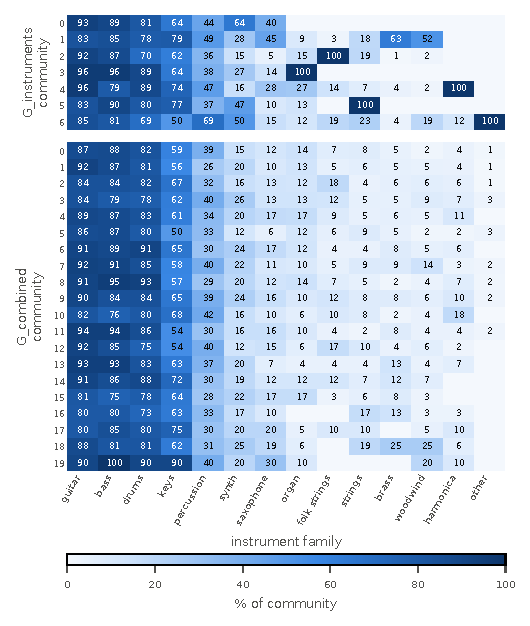
\includegraphics[width=\linewidth]{figures/report_instrument_profile.pdf}
  \caption{\textbf{Each instrument community is held together by one rare instrument family.} Share of each community's songs that has each instrument family (a song has several families, so rows do not sum to 100\%), for the \Ginst{} and \Gcomb{} communities. In \Ginst, folk strings (community 2), organ (3), harmonica (4), strings (5) and other instruments (6) are present on all songs of one community, while guitar, bass and drums are present on 69--96\% of the songs in all communities. The \Gcomb{} communities have no such marker family; the highest share is 18\% folk strings in community 2, which also has the most Canadian releases (58\%).}
  \label{fig:instruments}
\end{figure}

\subsection*{The combined graph is organized by release country}
In \Gcomb, release country explains the communities far better than genre (AMI 0.403 against 0.014; country assortativity 0.375). Five communities have 45--74\% of their songs from a single release country outside the US and GB (Fig.~2, right), and the backbone weight is 68\% words, 28\% country and only 4\% instruments, although the three types have equal weight before filtering. Reducing the weight of country removed this structure but did not reveal a genre structure behind it. At country weights of 1, 0.5, 0.25 and 0, the AMI with country fell from 0.403 to 0.135, 0.026 and 0.002, and the AMI with genre also fell, from 0.014 to 0.007, 0.003 and 0.008. Country thus carries part of the genre signal in \Gcomb{} rather than hiding it. For example, community 2, which draws 58\% of its songs from Canadian releases, also has the largest share of country music (16\%, baseline 4\%) and of folk strings (18\%). Lyrics alone hardly follow release country (AMI 0.007), and on the 673 common songs the agreement is not above chance ($p = 0.43$).

\subsection*{Lyrical themes}
The \Glyr{} communities are themes rather than genres. Their most distinctive words describe a conflict theme (``orders'', ``police'', ``bullets'', ``sheriff'', ``war''; 2,366 songs), a melancholic theme (``autumn'', ``sigh'', ``sorrows'', ``scattered''; 2,323 songs), a romance theme (``darlin'', ``squeeze'', ``lovin'', ``beggin''; 1,345 songs), a party theme (``mic'', ``mc'', ``disco'', ``microphone'', ``funk''; 856 songs), a barroom theme (``barroom'', ``husband'', ``tonk'', ``grave''; 463 songs) and a Christmas theme (``ding'', ``dong'', ``sleigh''; 328 songs). The romance and party themes have the most r\&b (34\% and 32\%, baseline 18\%). The mean song sentiment is low (VADER mean $0.09$, sd $0.14$). Communities explain 8.3\% of the sentiment variance in \Glyr{} ($\eta^2 = 0.083$, $p = 0.001$), against 4.1\% for genre ($\eta^2 = 0.041$, $p = 0.001$), and the differences are not significant in \Ginst{} ($p = 0.11$) or \Gcomb{} ($p = 0.076$). The romance theme has the highest median sentiment (0.139) and the conflict theme the lowest (0.035). The \Gcomb{} communities have no clear word themes, which agrees with their organization by country.

\subsection*{Associations between instrument, country and theme}
Of the 14 instrument families, five are associated with release country in both the chi-square and the permutation test after Bonferroni correction: folk strings ($V = 0.18$), keys ($V = 0.18$), bass ($V = 0.17$), guitar ($V = 0.12$) and strings ($V = 0.12$; all permutation $p_{\mathrm{Bonf}} \leq 0.042$, where 0.014 is the smallest possible value). All five associations are weak. The clearest is folk strings, which are 2.2 times more common than expected in Canadian releases, 1.7 times in US releases and 1.6 times in German releases, and half as common in British releases (lift 0.46; Fig.~4). Keys are less common in British releases (0.81), while the lifts of bass and guitar lie between 0.75 and 1.09; these associations are significant because of the many songs, not because of large differences. With the lyrical themes, only percussion passes both tests ($V = 0.12$, $p_{\mathrm{Bonf}} = 0.020$, permutation $p_{\mathrm{Bonf}} = 0.042$); percussion is less common in the conflict theme (0.80) and more common in the melancholic (1.16) and romance (1.14) themes. Folk strings are overrepresented in the barroom (1.7) and Christmas (1.6) themes, but these rest on 14 and 8 songs. The other lifts lie between 0.5 and 1.8.

\begin{figure}[t]
  \centering
  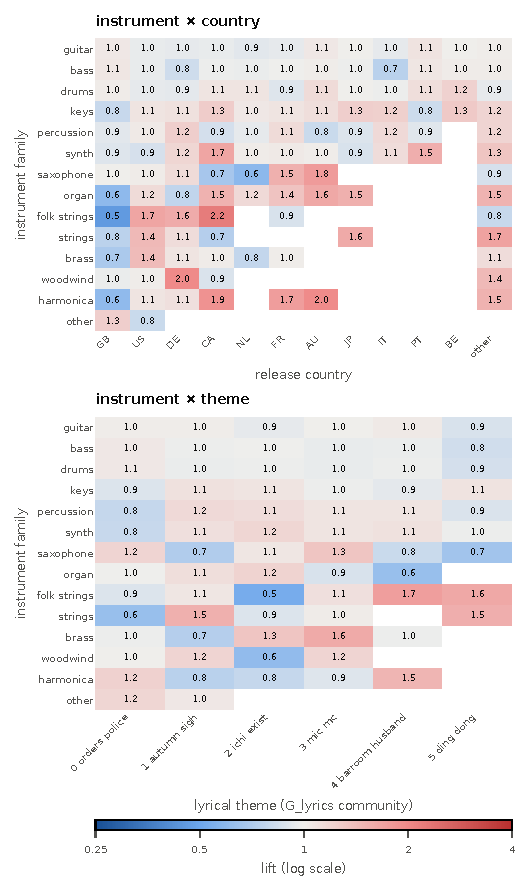
\includegraphics[width=\linewidth]{figures/report_lift.pdf}
  \caption{\textbf{Instrument families are largely independent of release country and lyrical theme, with folk strings as the clearest exception.} Lift $= P(A,B)/(P(A)P(B))$ between instrument family and release country (top, 2,171 songs, 11 countries plus other) and between instrument family and lyrical theme (bottom, the 6 \Glyr{} communities named by their two top words, 1,428 songs). Lift 1 (grey) means the family is as common as overall; red above, blue below, on a log scale. Cells with fewer than 5 songs are blank. After Bonferroni correction over 14 families, folk strings, keys, bass, guitar and strings are associated with country and percussion with theme in both the chi-square and the permutation test, but all with Cram\'er's $V \leq 0.18$.}
  \label{fig:lift}
\end{figure}

\begin{table}[t]
  \centering
  \caption{\textbf{Summary per graph.} Backbone LCC at $\alpha = 0.05$ and the Louvain partition with seed 42. $M_{\mathrm{null}}$: mean $\pm$ sd over 100 degree-preserving rewirings. AMI $p$-values from 1,000 label shuffles (minimum 0.001). Stability: mean pairwise AMI of 20 Louvain seeds.}
  \label{tab:summary}
  \small
  \begin{tabular}{lrrr}
    \toprule
     & \Glyr & \Ginst & \Gcomb \\
    \midrule
    Songs (LCC)            & 7,681 & 971 & 1,428 \\
    Edges                  & 992,571 & 54,248 & 46,399 \\
    Communities            & 6 & 7 & 20 \\
    $M$                    & 0.212 & 0.482 & 0.371 \\
    $M_{\mathrm{null}}$    & $0.055 \pm 0.001$ & $0.067 \pm 0.001$ & $0.180 \pm 0.001$ \\
    $z$                    & 184 & 337 & 195 \\
    Stability (AMI)        & 0.62 & 0.90 & 0.58 \\
    \midrule
    AMI genre ($p$)        & 0.033 (0.001) & 0.096 (0.001) & 0.014 (0.001) \\
    ARI genre              & 0.041 & 0.024 & 0.004 \\
    Assortativity genre    & 0.043 & 0.076 & 0.035 \\
    $M$ of genre partition & 0.033 & 0.047 & 0.020 \\
    \midrule
    AMI country ($p$)      & 0.007 (0.001) & 0.018 (0.001) & 0.403 (0.001) \\
    Assortativity country  & 0.010 & 0.008 & 0.375 \\
    \bottomrule
  \end{tabular}
\end{table}


% =====================================================================
\section*{Discussion}
% =====================================================================

Songs from 1970--1980 can be grouped into clusters that are clearly not random: all three networks have a modularity 184 to 337 standard deviations above degree-preserving null graphs. These clusters, however, correspond only weakly to established genres. Lyrics produce themes (conflict, melancholy, romance, partying, the barroom and Christmas) that cut across genres, with an AMI with genre of 0.033. Instrumentation comes closest to genre (AMI 0.096), but only through a few families that mark a style, such as folk strings for country and brass, woodwind and saxophone for r\&b and jazz. Combining lyrics, instruments and country does not improve the match with genre (AMI 0.014). Instead, the combined graph is organized by release country, and removing country lowers the genre agreement further. The answer to the research question is therefore that meaningful clusters exist, but they describe themes, instrument line-ups and release markets rather than genres.

The result does not show that lyrics are unrelated to genre. The agreement is small but well above every shuffle, and a partition into 6 communities can only capture the strongest lyrical divisions. A song can also share its theme with songs of any genre. The result also does not show that genre is a poor category in general. The genre labels are noisy: most MusicBrainz tags have a single vote, 69\% of the recordings with a genre carry the tags of their artist rather than their own, 427 genre labels were decided by a random draw between tied genres (Materials and Methods), and MusicBrainz and Genius agree on only 59\% of the songs labeled by both. Part of the low agreement may therefore come from the labels rather than from the networks. No hand-labeled sample was made to separate the two.

Several limitations come from the data. Rock is 57--79\% of the labeled songs, so genre agreement can say little beyond rock against the rest. Only 2,171 of the 25,491 songs (8.5\%) have instrument credits, and the backbone removes 1,200 of them because a standard rock line-up carries no distinguishing information. \Ginst{} therefore describes the 971 songs with a less common instrument, and its genre agreement may not hold for the songs that were dropped. Release country is the country of the earliest release, not the origin of the artist, so the country communities in \Gcomb{} partly reflect which national market a single was first released in.

Other limitations come from the methods. The combined and lyrics partitions are the least stable (seed AMI 0.58 and 0.62), so single communities of these graphs should not be interpreted song by song, although $M$ and the genre agreement hardly change between seeds. The null model keeps degrees but only keeps node strengths on average. Modularity has a resolution limit \cite{TODO_fortunato2007resolution}, so small genres such as jazz (41 songs with lyrics) or electronic (47) may be merged into larger communities. The top-10 TF-IDF words are only one way of representing a song's theme, and VADER scores words such as ``love'' as positive even in a sad song. A future study could test the labels against a hand-labeled sample, include more instrument credits (for example from Discogs), and use the artist's country instead of the release country.


% =====================================================================
\section*{Materials and Methods}
% =====================================================================

\subsection*{Songs analyzed}
The analysis covers English-language official singles first released 1970--1980 on MusicBrainz \cite{TODO_musicbrainz}, matched to lyrics from the Genius lyrics dataset on Kaggle \cite{TODO_genius_kaggle} (collection, cleaning and matching are described in [section by teammate]). After 23 duplicate lyrics were removed (spelling variants of the same title by the same artist, lyric cosine similarity $\geq 0.95$), the period contains 25,491 songs. Of these, 7,682 have lyrics, 2,171 have instrument credits and 1,428 have both. The release country of a song is the country of its earliest release, not the origin of the artist. All random steps use the seed 42, and every graph is put in sorted node order before a random step, because Louvain and the edge swaps otherwise depend on the order in which Python stores the song identifiers.

\subsection*{Genre labels}
MusicBrainz genres are user tags with a vote count. Most counts are small (61\% of the recording-tag counts are exactly 1), and 69\% of the recordings with a genre carry the tags of their artist, because the tags of the artist are used when a recording has none. Only tags on the official MusicBrainz genre list are kept. The labels were built in four steps:
\begin{itemize}
  \item \textbf{Votes.} The vote counts of each tag are summed over all recordings merged into one song.
  \item \textbf{Core genres.} Each label is reduced to the genre it is a kind of. English genre compounds put the main word last, so the shortest ending of the label that is itself a genre wins, with hyphens splitting words (``pop rock'' $\rightarrow$ rock, ``proto-punk'' $\rightarrow$ punk, ``west coast hip hop'' $\rightarrow$ hip hop). If no ending is a genre, the rightmost word that is a genre wins (``rock and roll'' $\rightarrow$ rock); otherwise the label is a core genre itself (``beat music'', ``singer-songwriter''). ``Rhythm and blues'' is always mapped to r\&b. This reduces 465 labels to 201 core genres.
  \item \textbf{Primary genre.} The votes are summed per core genre, and the most-voted core genre is the primary genre. Ties are drawn at random, seeded by the song identifier, so the draw is reproducible and does not depend on song order.
  \item \textbf{Evaluation genre.} Each core genre belongs to one coarse class (rock, pop, r\&b, country, folk, blues, jazz, reggae, electronic, rap or other), and the most-voted class is the evaluation genre. Classes with fewer than 30 songs with lyrics are merged into ``other''.
\end{itemize}
Each song therefore has two possible genre labels: its primary genre (one of 201 core genres) and its coarse class (one of 11 broad classes). The coarse class was chosen as the genre the communities are compared with, for three reasons. First, the research question asks about established genres, and these are the broad ones. Second, the primary genre separates subgenres that are almost the same, such as soul, r\&b, funk and disco. A community of soul and funk songs would then count as mixed, although it is one clear genre. Third, ties are less common between broad classes: among the 7,682 songs with lyrics, 427 coarse classes were decided by a random draw, against 982 primary genres. The primary genre is only used as a secondary check of the results. Among the songs with lyrics, the most common evaluation genre is rock (4,103 songs), followed by r\&b (1,320), pop (695) and country (637). Reggae (126), folk (122), electronic (47) and jazz (41) are smaller. Blues (22 songs) and rap (20 songs) fall below the limit of 30 songs and are part of ``other'' (92 songs in total). The remaining 499 songs with lyrics have no genre.

Genius also gives each song a genre tag, but this tag was not used for the evaluation. It only exists for songs with lyrics, and Genius uses ``pop'' as a catch-all: 1,707 songs that MusicBrainz labels as rock are tagged as pop on Genius. No genres were labeled by hand. The only check of the labels is therefore the agreement between the two sources, which is 59\% for the 7,056 songs that have a label from both.

\subsection*{Genre network}
As a first look at the labels, the 16,463 songs with at least one MusicBrainz genre were linked when their genre lists overlap, with the number of shared genres as edge weight. Each genre contributes at most 500 randomly sampled song pairs, so that rock does not dominate the graph. Communities were found with greedy modularity maximization \cite{TODO_clauset2004greedy}. Genre is used to build the edges of this graph, so it is only used to describe the labels and not to answer the research question.

\subsection*{Three song networks}
Songs are nodes in all three networks. Genre is never used to build an edge; it is only used afterwards, for evaluation.
\begin{itemize}
  \item \textbf{\Glyr} (7,682 songs). The lyrics were tokenized with spaCy \cite{TODO_spacy} ([tokenization by teammate]). Vocables and contraction fragments (``ooh'', ``yeah'', ``la'', ``gon''+``na'') were removed, which is 9.5\% of the tokens. TF-IDF vectors \cite{TODO_jurafsky_slp3} were computed with scikit-learn \cite{TODO_sklearn} with sublinear term frequency ($1+\ln$ count, so that a word repeated 40 times in a chorus weighs about 4.7 instead of 40), a minimum document frequency of 2 and a maximum document frequency of 0.5, giving 12,204 words. The edge weight is the cosine similarity between two songs. The full similarity graph is 87\% complete (25,756,510 edges) and is kept as a dense matrix until the backbone is extracted.
  \item \textbf{\Ginst} (2,171 songs). The 173 instrument names in the credits (35 of them on a single recording) were grouped into 14 families (drums, percussion, guitar, bass, keys, organ, synth, brass, saxophone, woodwind, strings, folk strings, harmonica, other), because many names describe the same role at different levels of detail (``bass'', ``bass guitar'', ``electric bass guitar''). The song--family bipartite graph was projected onto the songs with hyperbolic weighting \cite{TODO_newman2001hyperbolic}: a family shared by $k$ songs adds $1/(k-1)$ to each of their pairs. Guitar, bass and drums appear on 88\%, 86\% and 77\% of the songs and therefore add almost nothing to any pair.
  \item \textbf{\Gcomb} (1,428 songs with lyrics, instruments and country). Songs are linked through three feature types: instrument families, release country and the 10 words with the highest TF-IDF in each song. Each feature type is projected on its own with hyperbolic weighting, each projection is scaled to a total weight of 1, and the three are added, so that the three types have the same total weight. Without this balancing, the many rare words dominate: in a single projection of all features, words carried 96\% of the backbone weight.
\end{itemize}

\subsection*{Backbone extraction}
The three graphs are 87--95\% complete, so each was reduced to a backbone of significant edges before community detection. The disparity filter \cite{TODO_serrano2009disparity} was used, because the total edge weight differs strongly between songs and the filter judges each edge relative to the other edges of the same song. For an edge $(u,v)$ seen from song $u$, with strength $s_u$ (the sum of its edge weights) and degree $k_u$,
\begin{equation}
  p_u(u,v) = \left(1 - \frac{w_{uv}}{s_u}\right)^{k_u-1},
\end{equation}
is the probability that $u$'s strength, spread at random over its $k_u$ edges, gives one edge a weight of at least $w_{uv}$. An edge is kept if $p < \alpha$ from either endpoint ($\alpha = 0.05$), so it is enough that the edge stands out for one of the two songs. The single edge of a degree-1 node is always kept. \Glyr{} was filtered on its full similarity matrix. The implementation matched a direct edge-by-edge evaluation of the formula on 200-song test graphs at all three $\alpha$ values used. Community detection uses the largest connected component (LCC) of each backbone. The backbones are described by their degree distribution (complementary cumulative distribution on log-log axes, without a power-law fit) and by the average clustering coefficient, compared with an Erd\H{o}s--R\'enyi graph \cite{TODO_erdos1959random} of the same density and with the configuration-model expectation $C = (\langle k^2\rangle - \langle k\rangle)^2 / (\langle k\rangle^3 N)$ \cite{TODO_newman2003structure}.

\subsection*{Communities and their agreement with genre and country}
Communities were found with Louvain \cite{TODO_blondel2008louvain} (\texttt{networkx} \cite{TODO_networkx}), which maximizes the weighted modularity
\begin{equation}
  M = \frac{1}{2W}\sum_{ij}\left(w_{ij} - \frac{s_i s_j}{2W}\right)\delta(c_i,c_j)
\end{equation}
\cite{TODO_newman2004modularity, TODO_newman2004weighted}. The partitions were compared with the evaluation genre and with release country using only songs that have the label:
\begin{itemize}
  \item \textbf{Adjusted mutual information (AMI)} \cite{TODO_vinh2010ami} and \textbf{adjusted Rand index (ARI)} \cite{TODO_hubert1985ari}, which are corrected for chance, so that they are 0 for random agreement and 1 for identical partitions.
  \item \textbf{Attribute assortativity} \cite{TODO_newman2003assortativity} of the backbone edges, which measures whether links join songs with the same label more often than chance, independently of Louvain.
  \item \textbf{Modularity of the label partition}, i.e.\ $M$ with genre (or country) used as the communities, compared with Louvain's $M$ on the same songs.
  \item \textbf{Composition heatmaps}: the share of each label per community, next to the label shares of the whole LCC as baseline. Country is shown for the 8 most common release countries plus ``other''.
\end{itemize}
Because the three graphs contain different songs, AMI and ARI were also computed on the songs present in all three LCCs.

\subsection*{Validation}
\begin{itemize}
  \item \textbf{Configuration-model null for $M$.} Each backbone LCC was rewired 100 times with degree-preserving double edge swaps ($10|E|$ swaps) \cite{TODO_maslov2002rewiring}, the real weights were shuffled over the new edges, and Louvain was run on each null graph. The result is reported as a $z$-score and an empirical $p$-value, $(1 + \#\{M_{\mathrm{null}} \geq M\})/101$, whose minimum is 0.0099. Node strengths are only preserved on average under this procedure.
  \item \textbf{Permutation test for AMI.} With the communities fixed, the genre (or country) labels were shuffled over the songs 1,000 times, keeping the number of songs per label. The $p$-value is $(1+\#\{\mathrm{AMI}_{ \mathrm{null}} \geq \mathrm{AMI}\})/1001$, with minimum 0.001.
  \item \textbf{Seed stability.} Louvain was run with 20 seeds per graph, and the mean AMI over the 190 pairs of partitions is reported (1 = always the same partition).
  \item \textbf{Filter level.} The whole pipeline was repeated at $\alpha = 0.01$ and $0.1$.
  \item \textbf{Country weight.} \Gcomb{} was rebuilt with the country projection scaled by 0.5, 0.25 and 0, to test how much of the community structure and genre agreement depends on country.
\end{itemize}

\subsection*{Content of the communities}
Communities with at least 10 songs were described by their lyrics and instruments.
\begin{itemize}
  \item \textbf{Distinctive words.} Each community is one document. The term frequency counts how many of the community's songs use a word (once per song), so that a word repeated many times in a single song does not dominate, and IDF $= \log(\text{communities} / \text{communities using the word})$. Only words used by at least 5 songs of the graph are considered.
  \item \textbf{Sentiment.} VADER \cite{TODO_hutto2014vader} saturates at $\pm 1$ on a whole song, so each lyric line was scored on the raw text and a song's score is the mean compound score of its lines. Differences between communities, and between genres, were tested by shuffling song scores 1,000 times and comparing the between-group sum of squares; the effect size is $\eta^2$.
  \item \textbf{Instrument profile.} For \Ginst{} and \Gcomb, the share of each community's songs that has each instrument family.
\end{itemize}

\subsection*{Associations between instrument, country and theme}
The lyrical themes are the \Glyr{} communities, each named by its two most distinctive words. Instrument $\times$ country uses the 2,171 songs with instrument data, and instrument $\times$ theme the 1,428 of these with lyrics. Countries with fewer than 15 of these songs were grouped as ``other'', leaving 11 countries plus ``other''. Lift $= P(A,B)/(P(A)P(B))$ is shown on a log scale, and cells with fewer than 5 songs are left blank. Since a song usually has several instrument families, each family with at least 10 songs was tested in its own $2 \times K$ table (present/absent $\times$ the $K$ countries or themes) with a chi-square test, checked with a permutation $p$-value (1,000 shuffles) and Bonferroni-corrected for the number of families tested. Cram\'er's $V$ gives the strength of each association.

% ---------------------------------------------------------------------
% Placeholder citation keys used above:
%TODO_musicbrainz               MetaBrainz Foundation, MusicBrainz, https://musicbrainz.org [add date of the data download]
%TODO_genius_kaggle             Genius song lyrics dataset on Kaggle [check exact title, author and URL with the teammate who downloaded it]
%TODO_clauset2004greedy         Clauset, Newman & Moore 2004, Finding community structure in very large networks, Phys. Rev. E 70, 066111
%TODO_spacy                     Honnibal, Montani, Van Landeghem & Boyd 2020, spaCy: Industrial-strength natural language processing in Python, Zenodo, doi:10.5281/zenodo.1212303
%TODO_sklearn                   Pedregosa et al. 2011, Scikit-learn: Machine learning in Python, JMLR 12, 2825-2830
%TODO_newman2001hyperbolic      Newman 2001, Scientific collaboration networks. II. Shortest paths, weighted networks, and centrality, Phys. Rev. E 64, 016132
%TODO_serrano2009disparity      Serrano, Boguna & Vespignani 2009, Extracting the multiscale backbone of complex weighted networks, PNAS 106(16), 6483-6488
%TODO_blondel2008louvain        Blondel, Guillaume, Lambiotte & Lefebvre 2008, Fast unfolding of communities in large networks, J. Stat. Mech. P10008
%TODO_networkx                  Hagberg, Schult & Swart 2008, Exploring network structure, dynamics, and function using NetworkX, Proc. 7th Python in Science Conference (SciPy 2008), 11-15
%TODO_newman2004modularity      Newman & Girvan 2004, Finding and evaluating community structure in networks, Phys. Rev. E 69, 026113  [also on the course site, week 4]
%TODO_newman2004weighted        Newman 2004, Analysis of weighted networks, Phys. Rev. E 70, 056131  (weighted form of M)
%TODO_jurafsky_slp3             Jurafsky & Martin, Speech and Language Processing, 3rd ed. draft, https://web.stanford.edu/~jurafsky/slp3/  (course textbook; TF-IDF and cosine similarity in Ch. 11)
%TODO_erdos1959random           Erdos & Renyi 1959, On random graphs I, Publicationes Mathematicae Debrecen 6, 290-297
%TODO_newman2003structure       Newman 2003, The structure and function of complex networks, SIAM Review 45(2), 167-256  (clustering of the configuration model)
%TODO_vinh2010ami               Vinh, Epps & Bailey 2010, Information theoretic measures for clusterings comparison: Variants, properties, normalization and correction for chance, JMLR 11, 2837-2854
%TODO_hubert1985ari             Hubert & Arabie 1985, Comparing partitions, Journal of Classification 2, 193-218
%TODO_newman2003assortativity   Newman 2003, Mixing patterns in networks, Phys. Rev. E 67, 026126
%TODO_maslov2002rewiring        Maslov & Sneppen 2002, Specificity and stability in topology of protein networks, Science 296(5569), 910-913
%TODO_hutto2014vader            Hutto & Gilbert 2014, VADER: A parsimonious rule-based model for sentiment analysis of social media text, Proc. ICWSM 8(1), 216-225
%TODO_fortunato2007resolution   Fortunato & Barthelemy 2007, Resolution limit in community detection, PNAS 104(1), 36-41
% ---------------------------------------------------------------------
